\mytitle{A Física dos Esportes}    
\addchaptersummary{A Física dos Esportes}{Sumario/Figs_Sumario/FigArtigo4.jpg}{Na cabeça de muitos, Física e Esportes nunca andaram lado a lado, mas a grande verdade é que eles tem tudo a ver. Você pode achar que não, mas já fez muita conta de cabeça numa partida de futebol!}{Vítor Hugo Ribeiro} 
\newcommand{\artigoquatro}{\begin{center}\textcolor{base}{\MakeUppercase{A Física dos Esportes}}\end{center}}

\begin{figure}[H]
		\centering
		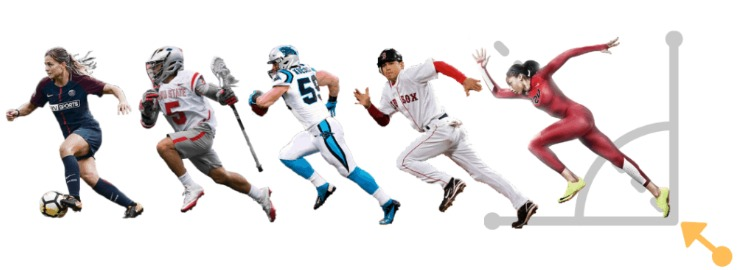
\includegraphics[width=0.95\linewidth]{Figuras/Artigo4/esportes.jpeg}
		\caption{As leis Físicas estão presentes, sem exceção, em todos os esportes. [Fonte:  \href{https://velocityspusa.com/myth-or-fact-speed-training-is-sport-specific/}{velocityspusa}].}
		\label{fig:v1}
	\end{figure}

\begin{multicols}{2}

A história da Física se inicia na antiguidade, quando as pessoas, por algum motivo, começaram a se perguntar os ``porquês'' das coisas. Ou melhor ainda, falando isso de uma maneira um pouco mais específica, começaram a se perguntar a respeito da natureza e suas interações, tentando entender os conceitos por trás destes elementos, sem que houvesse a necessidade de algo místico para explicá-los. E agora, no momento atual, você deve estar se perguntando o que isso tem a ver com o título desse texto, visto que eu sequer citei o termo ``Esporte'' nessa introdução. Pois bem, respondendo a sua pergunta, é interessante começar com essa introdução histórica pois foram nesses momentos iniciais da Física que surgiram os primeiros pensamentos a respeito do movimento e de como descrevê-lo. Nesse contexto, também não existe palavra melhor para se referir aos esportes do que movimento. Esportes são caracterizados por seres em movimento e a Física foi a primeira ciência que se preocupou em estudá-los.
 
Apesar dessa relação intrínseca entre os termos Física e Esportes para com a palavra movimento, hoje em dia não se vê uma conexão direta entre os três. Na verdade, o que podemos notar é uma relação um tanto quanto oposta, demonstrada no fato de que muitos alunos, no geral, preferem as aulas de Educação Física do que as de Física ou Matemática. É claro que esse tipo de comparação não é justa, visto que diversos outros fatores interferem nessa escolha, mas o ponto principal que pretendo trazer aqui é que dificilmente as pessoas associam os esportes com pensamentos e conceitos Físicos. Nos esportes, tudo é mais dinâmico e intuitivo, não é necessário fazer cálculos para se chegar a um resultado e, por isso, talvez, a aula de Educação Física seja a preferida. No entanto, ao mesmo tempo, realizar um determinado movimento exige preparação física e psicológica para que ele seja executado da maneira correta. Dessa forma, pode até não parecer, mas isso exige diversos raciocínios físicos e aproximações que são calculadas de maneira instintiva e que culminam naquele golaço do camisa 10 no gol do time adversário. 
 Talvez seja exatamente por não enxergar esse tipo de relação, que as pessoas sintam um pouco de medo da Física e achem-na muito difícil. Quando se fala nesta disciplina, todo mundo se lembra das equações que estudava, ou na verdade, lembram que havia muitas equações, mas dificilmente se lembram dos conceitos por trás delas. Ideias como força e velocidade são comuns no nosso dia a dia e, no geral, todo mundo sabe ou tem uma noção mínima do que significam. Porém, quando partimos para conceitos como potência e trabalho, altamente relacionados com atividades esportivas, as pessoas não têm ideia de como explicá-los, embora cheguem a discutir ideias relacionadas a eles quando veem o movimento de um atleta numa modalidade olímpica. Além disso, ao realizar tal análise, as pessoas lidam com situações muito mais complicadas do que aquelas estudadas nas aulas de Física, em que o atrito era desprezível e todo o resto constante. Quando avaliamos uma situação na realidade, assim como nos esportes, nada é constante, ou melhor ainda, tudo está em constante mudança. Nesse sentido é um tanto quanto interessante observar que as pessoas sentem mais interesse em estudar uma situação complicada como esta do que uma situação simples como aquelas abordadas em salas de aula. Mas aqui, novamente, diversos fatores devem ser levados em consideração para justificar esse tipo de escolha. Talvez o mais importante deles é que nestas discussões a matemática não é a ferramenta principal, mas somente um guia que nos ajuda a ter uma noção de proporção, encaminhando a análise para algo que faça sentido. A nossa capacidade de avaliar proporções diretas ou indiretas e relacioná-las com aproximações torna tudo isso mais simples e configura o cerne dessa nossa conversa.
    
Para trabalhar um pouco disso, vamos revisar estes conceitos e ver como estas ideias se aplicam de maneira prática. Uma forma interessante de fazer isso é realizando a análise de duas modalidades olímpicas muito parecidas, mas também, ao mesmo tempo, muito diferentes: os $100$m rasos e a maratona. Numa corrida, tudo que citamos está sendo aplicado: velocidade, força, trabalho, potência e ainda algumas coisas a mais. Porém vamos focar nestes 4 primeiros. Os alvos de nosso estudo serão os dois medalhistas de ouro que venceram as modalidades de Maratona e $100$m rasos na Olimipíada do Rio de Janeiro, em 2016. Enquanto, na primeira modalidade, o corredor percorre uma distância total de $42$km, na segunda, o velocista percorre $100$m. Em ambas o objetivo é o mesmo: chegar primeiro. Porém, podemos ver de maneira nítida a diferença entre as duas: a primeira apresenta uma distância a ser percorrida que é $420$x maior que a segunda.

Os dados que vamos utilizar serão apenas três: a distância da prova, o tempo em que essa distância foi percorrida e a energia gasta para percorrê-la. Veja abaixo os dados de cada modalidade:


\begin{figure}[H]
    \centering
    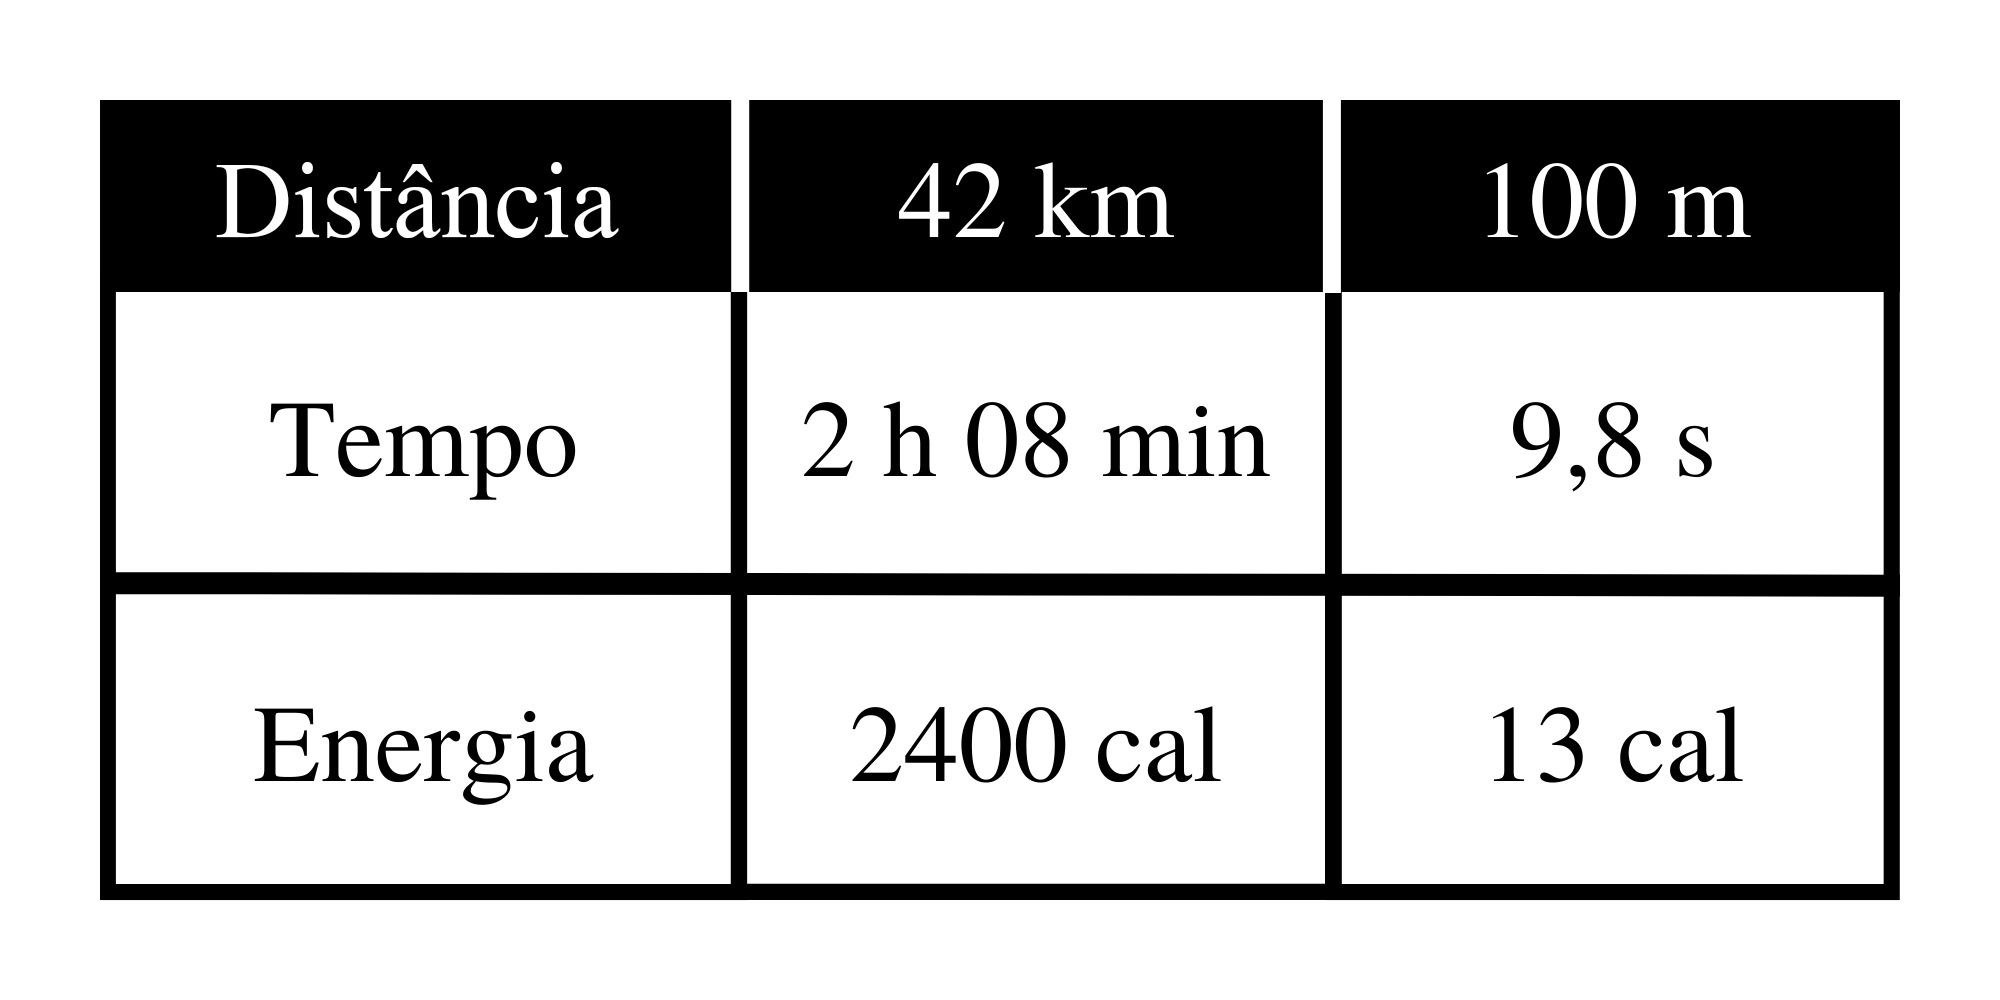
\includegraphics[width=\linewidth]{Figuras/Artigo4/tabela.jpg}
    \caption{Tais dados levam em conta estimativas de gastos calóricos que não correspondem de maneira exata com a realidade, mas que servem como uma forma de aproximação mais do que suficiente para realizarmos nossos cálculos.}
    \label{corredores}
\end{figure}

Tendo essas informações em mãos, podemos começar nossa análise. Primeiramente, iremos avaliar cada ponto utilizando como base nossa intuição e bom senso, para depois confirmarmos essa ideia através de alguns cálculos matemáticos. Essa pode até parecer uma prática simplista, visto que nessa etapa não utilizaríamos nenhum conceito complexo para chegar a conclusão final. Mas a ideia é exatamente essa, tentar chegar a uma conclusão apenas utilizando nossas noções básicas do mundo que nos cerca.

O primeiro tópico a ser estudado será a velocidade, ou seja, pretendemos avaliar a rapidez com que os dois atletas completam a prova e chegar a conclusão de qual deles apresenta uma maior velocidade. Nesse ponto, não é segredo pra ninguém que, de longe, o velocista que percorre apenas $100$ m apresentará uma velocidade muito maior que o maratonista. Não há uma justificativa direta para isso, de maneira que possamos escrevê-la aqui, apenas o bom senso. Uma forma de afirmar esse resultado pode ser dado observando alguns vídeos e comparando o ritmo de corrida de ambos os atletas. Agora, para confirmar essa análise por meios matemáticos, façamos o cálculo da velocidade média deles ao longo da prova. Para isso, aplicaremos uma equação, que é um tanto quanto intuitiva, e suas devidas conversões:

\begin{equation*}
    V_{m} = \dfrac{\text{distância}}{\text{tempo}}
\end{equation*}

\noindent\textbf{Maratonista:}\par % Use \par para criar um novo parágrafo, que é o equivalente explícito de deixar uma linha em branco. Evitando assim o erro underfull \hbox que ocorre quando o compilador não consegue ajustar o texto de forma ideal dentro de uma caixa horizontal

$V_m = \dfrac{42 \: \: \text{km}}{2\: \text{h} \: 08 \: \text{min}} \approx  5,5$ m/s

\noindent\textbf{Velocista:}\par

$V_m = \dfrac{100 \text{m}}{9,8} \approx 10,2$ m/s

Perceba que os dois resultados foram bem diferentes, como era de se esperar, e também concordaram com a análise prévia que havíamos feito. Enquanto o maratonista corre com uma velocidade de cerca de $5,5$ m/s o velocista corre com uma velocidade que é praticamente o dobro daquela apresentada pelo maratonista.

Seguindo por essa linha de raciocínio, podemos utilizar este resultado e inferir a força que cada atleta deve aplicar através dos músculos para alcançar essa velocidade. Tal ideia pode vir com um argumento muito simples: como o corredor de $100$ m rasos atinge uma velocidade maior em menos tempo, provavelmente ele deve fa zer muito mais ``força nas pernas'' para alcançar tal velocidade. Nesse caso, para realizar o cálculo matemático e comprovar, ou não, a nossa análise, utilizaremos uma pequena aproximação. Levaremos em conta que o tempo necessário para o velocista atingir sua velocidade máxima seja de aproximadamente $4,5$ s, ou seja, pouco menos de metade do tempo da prova. Agora, perceba, que não podemos utilizar o mesmo intervalo de tempo para o maratonista, visto que o mesmo não tem a necessidade de acelerar tudo de uma vez logo no começo. Por isso, para fins de aproximação, consideraremos que o maratonista terá cerca de $3$ min para alcançar sua velocidade de prova. Então, utilizando a equação para calcular a aceleração média esses atletas no intervalo de tempo escolhido, temos os seguintes resultados:

\begin{equation*}
    A_{m} = \dfrac{\text{velocidade}}{\text{tempo}}
\end{equation*}

\noindent\textbf{Maratonista:}\par

$A_m = \dfrac{5,5 \: \: \text{m/s}}{3 \: \text{min}} \approx  0,03$ m/$\text{s}^2$

\noindent\textbf{Velocista:}\par 

$A_m = \dfrac{10,2 \text{m/s}}{9,8 \: \text{s}} \approx 1,04$ m/$\text{s}^2$

Ou seja, como podemos observar, a aceleração do velocista é quase $35$x maior do que a aceleração do maratonista. O que, quando colocado em termos de força, que de acordo com a Segunda Lei de Newton é calulada como sendo a massa multiplicada pela aceleração, obteríamos o seguinte:

\noindent\textbf{Maratonista:}\par

$F = (60 \: kg) \times  0,03$ m/$\text{s}^2$ = $1,8 \: N$

\noindent\textbf{Velocista:}\par

$F = (80 \: kg) \times  1,04 $ m/$\text{s}^2$ = $83,2 \: N$

Nesse ponto, também fizemos uma pequena aproximação nas massas de cada atleta, mas veja que o nosso resultado continuou o mesmo. O velocista de $100$m rasos executa uma força muito mais intensa para alcançar o final da prova do que o corredor de maratona. Mas aqui, vale uma ressalva muito grande. Perceba que eu falei ``força muito mais intensa'', me referindo somente ao valor da força que foi aplicada no momento da aceleração. Mas quando falamos do corpo humano, para que ele permaneça em movimento, as pernas precisam continuar executando força. Assim, enquanto após os $9,8$ s de prova do velocista ele pode parar e descansar, o maratonista, por sua vez, precisa continuar aplicando sua força para permanecer em movimento, e pior ainda, um movimento de mais de $2$ horas.

Essa grande diferença no tempo de aplicação de uma força nos conecta diretamente ao quarto conceito que será abordado nessa revisão, o conceito de Potência. Porém, antes de chegar até ele, precisamos ter uma ideia do que significa Trabalho. Na Física, de maneira simples, Trabalho nada mais é do que a energia gasta para realizar um determinado movimento. Em nosso caso, tal conceito está relacionado a quantidade de calorias gastas pelo atleta para completar a prova em questão. Nesse caso, não sobra muito espaço para realizarmos uma análise inicial, visto que estes valores já foram dados previamente. Porém, isso ainda deve fazer sentido para nós que estamos estudando as duas situações. Enquanto o velocista realiza sua prova em menos de $10$ s, o maratonista passa cerca de $2$ horas correndo e, se deixarmos o ``bom senso'' nos guiar, facilmente poderíamos afirmar que o maratonista gasta mais energia para correr ao longo de sua prova do que o velocista. Ainda, nesse ponto, também não há um cálculo que confirme isso, já que pela informação da tabela já possuímos exatamente o valor associado ao trabalho. Logo nesse caso, nos demos bem.

Por fim, abordando agora o quarto conceito, podemos relacionar a discussão exercida quando falamos de força com a ideia de trabalho. No contexto que estamos abordando, o corredor de maratona exerce uma força através de suas pernas por um período de mais de $2$ horas, enquanto que o velocista dos $100$ m rasos, completa a modalidade em menos de $10$ s. Avaliando o tempo em que as provas são realizadas, torna-se difícil classificar o movimento dos atletas no sentindo de a quantidade total de força aplicada. Dessa forma, para contornar esse problema, podemos levar em conta o conceito de potência, que está associado a energia consumida num determinado intervalo de tempo. Tal ideia representa a eficiência com que a energia é gasta num determinado movimento, de forma que quanto mais energia é gasta num menor intervalo de tempo, mais potente seria esse movimento. Com base nessa descrição e utilizando um pouco de conhecimento comum, poderíamos dizer que o velocista apresenta uma potência maior, visto que ele acelera mais e alcança uma velocidade maior num intervalo de tempo menor. Ou seja, o seu movimento é muito eficiente no sentido de alcançar grandes resultados rapidamente. Ao mesmo tempo, o maratonista desenvolve uma prova muito mais longa e apesar de consumir muito mais energia, apresenta resultados menores. Para confirmar então essa análise, poderíamos calcular a potência entre os atletas de ambas as modalidades considerando a seguinte equação:

\begin{equation*}
    P_{m} = \dfrac{\text{trabalho}}{\text{tempo}}
\end{equation*}

\noindent\textbf{Maratonista:}\par

$V_m = \dfrac{2400\: \: \text{cal}}{2\: \text{h} \: 08 \: \text{min}} \approx  0,31$ cal/s

\noindent\textbf{Velocista:}\par

$V_m = \dfrac{13 m}{9,8} \approx 1,33$ cal/s

Por meio desses resultados, podemos concluir que um atleta de $100$ m rasos apresenta uma potência de movimento que é cerca de $4$x maior do que a de um maratonista. Também, analisando este resultado, verifica-se que ele faz sentido, visto que um corredor aplica toda a sua força e energia para conseguir atingir a linha de chegada dos $100$ m primeiro, de forma que esta é uma distância curta, então movimentos explosivos e com altas velocidades acabam sendo vantajosos. Ao mesmo tempo, um maratonista não deseja aplicar toda a sua força e energia nos primeiros instantes do trajeto, pois, caso isso aconteça, ele se esgotará muito rápido e não terminará o percurso. Logo, a estratégia de uma maratonista é equilibrar a aplicação de força e velocidade com gasto energético de forma a aumentar a eficiência da sua corrida. 

Ambas as modalidades estudadas aqui são completamente diferentes. Exigem treinos e estratégias diferentes. Mas são excelentes exemplos para entender os conceitos de velocidade, força, trabalho e potência.  Além dessas diferenças conceituais em termos relacionadas a física básica, também podemos descrever diferenças importantes no que diz respeito a biofísica do movimento. Por exemplo, observe a foto abaixo, em que comparamos um atleta de maratona com um atleta de atletismo que corre os $100$ m rasos.

\begin{figure}[H]
    \centering
    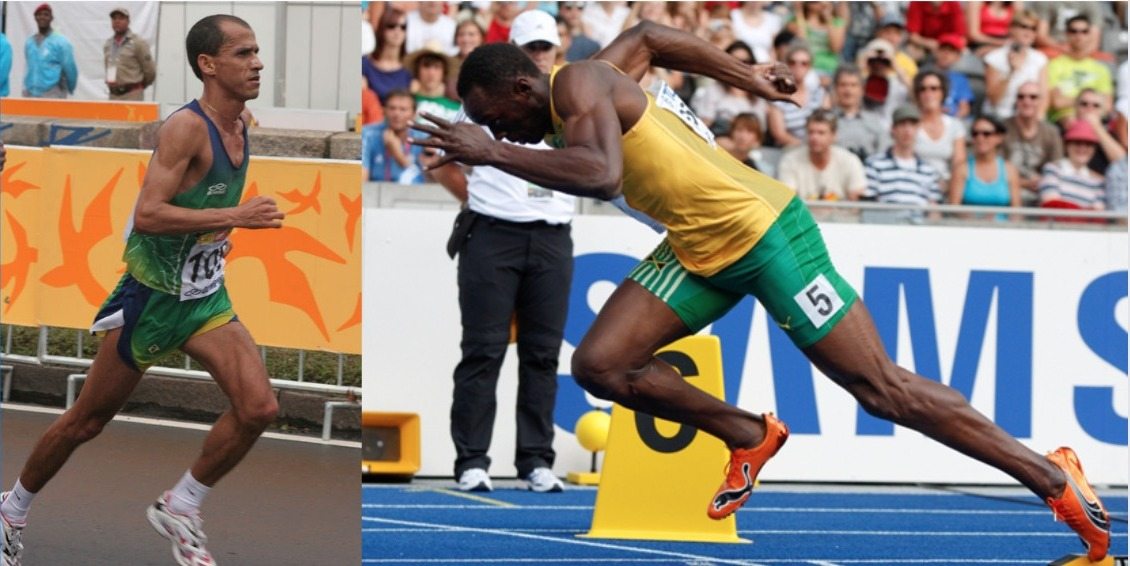
\includegraphics[width=\linewidth]{Figuras/Artigo4/corredores.jpeg}
    \caption{A esquerda, o maratonista Vanderlei Cordeiro de Lima. A direita o velocista Usain Bolt. [Fonte:  \href{https://museuescola.ibb.unesp.br/subtopico.php?id=2&pag=2&num=3&sub=25}{Museu Escola}]}
    \label{corredores2}
\end{figure}

Note que os músculos do corredor de $100$ m rasos são bem maiores e mais desenvolvidos do que os músculos do maratonista. Isso está diretamente ligado à potência que o músculo pode desenvolver. Dentro da fisiologia de um músculo, quando queremos algo com maior eficiência em tempos curtos, ou seja, movimentos explosivos, a melhor estrutura é alcançada com fibras que quando fortalecidas ficam mais grossas, aumentando o volume do músculo de maneira significativa. Enquanto isso, quando se tem como objetivo realizar movimentos de intensidade moderada por um longo período de tempo, a estratégia é que o músculo seja resistente e capaz de aplicar um força por um tempo bem maior. Nesse caso, a estrutura muscular que alcança esse resultado é aquela com fibras que mesmo fortes não variam muito de tamanho, como podendo ser observado na perna do corredor de maratonas.

Toda a análise realizada aqui foi uma grande aproximação para que eu tentasse demonstrar a você, caro leitor, essa conexão entre Física e Esportes. Por meio da aplicação de conceitos básicos relacionados à Física, podemos desenvolver nosso entendimento sobre as modalidades esportivas e assim aumentar muito mais a nossa percepção sobre movimentos e jogadas que muitas vezes parecem impossíveis. Não é necessário que tudo seja regrado fixamente pela matemática, afinal, como já foi dito, somos capazes de realizar cálculos ``de cabeça'' de uma maneira muito dinâmica através de aproximações e experiências. É exatamente isso que um atleta faz ao lançar uma bola de basquete, ele calcula a força e o ângulo necessário para que ao efetuar a jogada, a bola caia exatamente no centro do aro que configura a cesta e assim marca o ponto para o seu time. Usando esses métodos, somos capazes de entender não só um pouco mais de Física e de Esportes, como também de vários outros aspectos do mundo que nos cerca, basta um pouco de curiosidade e interesse, assim como é com esse amor mundial pelos esportes.

\authorinfo{Vítor Hugo Ribeiro}{http://lattes.cnpq.br/3783591692429936}


\end{multicols}